\documentclass[border=10pt]{standalone}
\usepackage{pgfplots}
\usepackage{sansmath}
\pgfplotsset{tick label style = {font=\sansmath\sffamily}}
\begin{document}
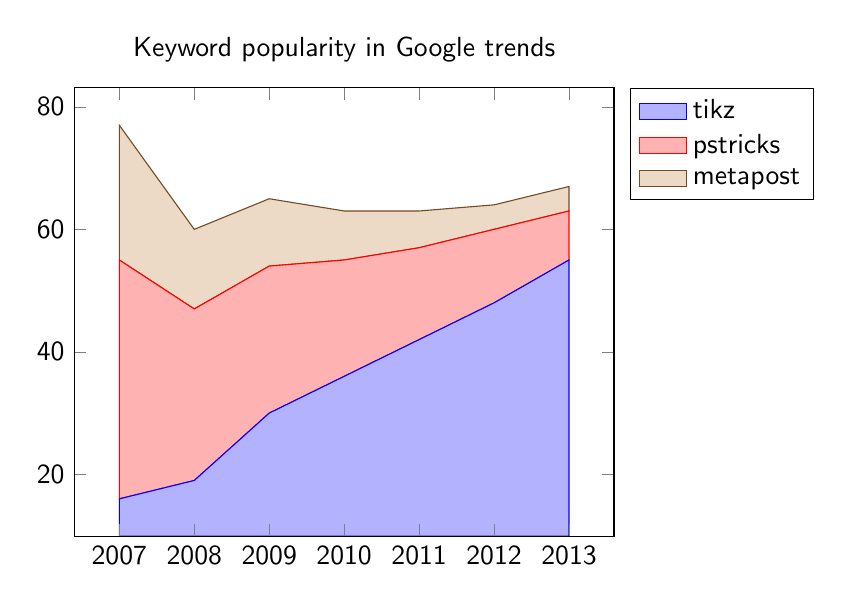
\begin{tikzpicture}[every node/.style={font=\sffamily}]
  \begin{axis}[title  = Keyword popularity in Google trends,
    stack plots=y,
    area style,
    x tick label style =
      {/pgf/number format/set thousands separator={}},
    legend pos = outer north east,
    legend cell align=left ]
  \addplot coordinates { (2007,16) (2008,19) (2009,30) (2010,36)
    (2011,42) (2012,48) (2013,55)}\closedcycle;;
  \addplot coordinates { (2007,39) (2008,28) (2009,24) (2010,19)
    (2011,15) (2012,12) (2013,8)}\closedcycle;;
  \addplot coordinates { (2007,22) (2008,13) (2009,11) (2010,8)
    (2011,6) (2012,4) (2013,4)}\closedcycle;;
  \legend{tikz, pstricks, metapost}
  \end{axis}
\end{tikzpicture}
\end{document}
